\documentclass[uplatex,dvipdfmx,a4paper,8pt]{jsarticle}
\usepackage{graphicx}
\usepackage{amsmath}
\usepackage{latexsym}
\usepackage{multirow}
\usepackage{url}
\usepackage[separate-uncertainty]{siunitx}
\usepackage{physics}
\usepackage{enumerate}
\usepackage{bm}
\usepackage{pdfpages}
\usepackage{pxchfon}
\usepackage{tikz}
\usepackage{float}
\usepackage{listings}
\usepackage{multicol}

% lstlistingのsetting
\lstset{
    basicstyle={\tiny\ttfamily},
    identifierstyle={\tiny},
    commentstyle={\tiny\itshape},
    keywordstyle={\tiny\bfseries},
    ndkeywordstyle={\tiny},
    stringstyle={\tiny\ttfamily},
    frame={tb},
    breaklines=true,
    columns=[l]{fullflexible},
    numbers=left,
    xrightmargin=0zw,
    xleftmargin=1zw,
    numberstyle={\scriptsize},
    stepnumber=1,
    numbersep=0.5zw,
    lineskip=-0.5ex
}

% tikz setting
\usepackage{tikz}
\usetikzlibrary{automata, intersections, calc, arrows, positioning, arrows.meta}

% theories setting (for japanese language)
\usepackage{amsmath}
\usepackage{amsthm}

\theoremstyle{definition}
\newtheorem{thm}{定理}[section]
\newtheorem{lem}[thm]{補題}
\newtheorem{prop}[thm]{命題}
\newtheorem{cor}[thm]{系}
\newtheorem{ass}[thm]{仮定}
\newtheorem{conj}[thm]{予想}
\newtheorem{dfn}[thm]{定義}
\newtheorem{rem}[thm]{注}

\newtheorem*{thm*}{定理}
\newtheorem*{lem*}{補題}
\newtheorem*{prop*}{命題}
\newtheorem*{cor*}{系}
\newtheorem*{ass*}{仮定}
\newtheorem*{conj*}{予想}
\newtheorem*{dfn*}{定義}
\newtheorem*{rem*}{注}

% \renewcommand{\rmdefault}{pplj}
% \renewcommand{\sfdefault}{phv}

\setlength{\textwidth}{190mm}
\setlength{\marginparwidth}{10mm}
\setlength{\textheight}{265mm}
\setlength{\topmargin}{-15mm}
\setlength{\oddsidemargin}{-10mm}
\setlength{\evensidemargin}{-10mm}
\setlength{\parindent}{0pt}
\setlength{\parskip}{1pt}
\setlength{\columnsep}{3mm}

\def\vector#1{\mbox{\boldmath $#1$}}
\newcommand{\AmSLaTeX}{%
 $\mathcal A$\lower.4ex\hbox{$\!\mathcal M\!$}$\mathcal S$-\LaTeX}
\newcommand{\PS}{{\scshape Post\-Script}}
\def\BibTeX{{\rmfamily B\kern-.05em{\scshape i\kern-.025em b}\kern-.08em
 T\kern-.1667em\lower.7ex\hbox{E}\kern-.125em X}}
\newcommand{\DeLta}{{\mit\Delta}}
\renewcommand{\d}{{\rm d}}
\def\wcaption#1{\caption[]{\parbox[t]{100mm}{#1}}}
\def\rm#1{\mathrm{#1}}
\def\tempC{^\circ \rm{C}}

\makeatletter
\def\section{\@startsection {section}{1}{\z@}{-2ex plus -0.5ex minus -.1ex}{1ex plus .1ex}{\normalsize\bf}}
\def\subsection{\@startsection {subsection}{2}{\z@}{-1.5ex plus -0.5ex minus -.1ex}{0.5ex plus .1ex}{\small\bf}}
\def\subsubsection{\@startsection {subsubsection}{3}{\z@}{-1ex plus -0.5ex minus -.1ex}{0.3ex plus .1ex}{\footnotesize\bf}}
\makeatother

\makeatletter
\def\@seccntformat#1{\@ifundefined{#1@cntformat}%
   {\csname the#1\endcsname\quad}%      default
   {\csname #1@cntformat\endcsname}%    enable individual control
}

% proof enviroment
\renewenvironment{proof}[1][\proofname]{\par
  \pushQED{\qed}%
  \normalfont \topsep6\p@\@plus6\p@\relax
  \trivlist
  \item\relax
  {\bfseries
  #1\@addpunct{.}}\hspace\labelsep\ignorespaces
}{%
  \popQED\endtrivlist\@endpefalse
}
\makeatother

\newcommand{\tenexp}[2]{#1\times10^{#2}}


\begin{document}
\small % 基本の文字サイズを小さく
\begin{multicols*}{4}
% 列のバランスを取らずに順次埋める

\section{必須課題}
\subsection{問題1}
\begin{itemize}
    \item 許容解: 最適化問題において、集合\(S\)の要素\(\bm{x}\)のこと。
    \item 目的関数: 最適化問題において、最大化したい関数\(f(\bm{x})\)のこと。
    \item 最適解: 任意の\(\bm{x} \in S\)に対して\(f(\bm{x}) \geq f(\bm{x}^*)\)となる許容解\(\bm{x}^*\)のこと。
    \item 最適値: 目的関数値の上界の最小値。
\end{itemize}

\subsection{問題2}
\subsubsection{(a)}
\hspace{1em}\((x, y) = (6, -6)\)を条件式の左辺に代入して計算すると

\begin{equation}
    3 \times 6 +2 \times (-2) = 6
\end{equation}

\noindent となり、条件式の右辺の値に一致するため\((6, -6)\)はこの最適化問題の許容解である。

\subsubsection{(b)}
\hspace{1em}\((x, y) = (0, 3)\)とすると、\(0^2 + 3^2 = 9\)で目的関数値をとり、かつ\(3 \times 0 + 2 \times 3 = 6\)で条件も満たすため、これが題意を満たす許容解の1つである。

\subsubsection{(c)}
\hspace{1em}\(x^2 + y^2  = k^2\)とおくと、最適化問題は条件\(3x + 2y = 6\)を満たしたうえで\(k^2\)を最小化するような\(\bm{x}\)を見つける問題になる。 \\
\hspace{1em}さて、\(x^2 + y^2 = k^2\)は\(x-y\)平面上の原点中心で半径が\(k\)の円を表している。
したかって求める\(k\)の値は原点から直線\(3x + 2y = 6\)への距離の値に等しい。
点と距離の直線公式を用いると\(k\)の値は

\begin{align}
    k   &= \frac{|3 \times 0 + 2 \times 0 - 6|}{\sqrt{3^2 + 2^2}} \\
        &= \frac{6}{\sqrt{13}}
\end{align}

\noindent であるから最適値は\(k^2 = \frac{36}{13}\)と求まる。 \\
\hspace{1em}次に最適値を与える最適解を求める。
最適解を求めるには以下の連立方程式を解けば良い。

\begin{equation} 
    \left\{ \,
        \begin{aligned}
            &   x^2 + y^2 = \frac{36}{13} \\
            &   3x + 2y = 6
        \end{aligned}
    \right.
\end{equation}

\noindent 2つ目の式を\(y\)について整理して1つ目の式に代入すると\(x\)は次のように求まる。

\begin{align}
    x^2 + \left(-\frac{3}{2}x + 3\right)^2  &= \frac{36}{13}    \\
    \left(x - \frac{18}{13}\right)^2        &= 0                \\
    x                                       &= \frac{18}{13}
\end{align}

\noindent 次に連立方程式の2式目に得られた\(x\)の値を代入して\(y\)の値を求めると\(y = \frac{12}{13}\)となる。
よって、最適解は\(\left(x, y\right) = \left(\frac{18}{13}, \frac{12}{13}\right)\)となる。

\subsection{問3}
\hspace{1em}(b)がありえない。

\subsection{問4}
\subsubsection{定式化}
\hspace{1em}製品Ⅰを\(x\)単位、製品Ⅱを\(y\)単位生産すると設定すると、最適化問題は以下のように定式化できる。

\begin{equation}
    \left\{ \,
        \begin{aligned}
            & \text{目的関数: } 3x + 2y \\
            & \text{条件1: } 5x + y \leq 10 \\
            & \text{条件2: } x + 2y \leq 5 \\
            & \text{条件3: } x, y \geq 0
        \end{aligned}
    \right.\
\end{equation}

\subsubsection{実行可能領域の図示}
\hspace{1em}以上の定式化をもとにこの最適化問題の実行可能領域を図示すると以下のようになる。

\begin{figure}[H]
    \centering
    \begin{tikzpicture}[scale=1.5]
        % 軸の描画
        \draw[->] (-0.5,0) -- (3,0) node[right] {$x$};
        \draw[->] (0,-0.5) -- (0,3) node[above] {$y$};
        
        % グリッド
        \draw[help lines, gray!30] (0,0) grid (3,3);
        
        % 制約条件の直線
        % 条件1: 5x + y = 10 → y = 10 - 5x
        \draw[thick, blue] (1.4,3) -- (2,0) node[pos=0.5, above left] {$5x + y = 10$};
        
        % 条件2: x + 2y = 5 → y = (5-x)/2
        \draw[thick, red] (0,2.5) -- (3,1) node[pos=0.6, below right] {$x + 2y = 5$};
        
        % 実行可能領域の塗りつぶし
        \fill[green!20, opacity=0.5] (0,0) -- (0,2.5) -- (1.667,1.667) -- (2,0) -- cycle;
        
        % 頂点の描画
        \fill (0,0) circle (2pt) node[below left] {$(0,0)$};
        \fill (0,2.5) circle (2pt) node[left] {$(0,2.5)$};
        \fill (2,0) circle (2pt) node[above] {$(2,0)$};
        \fill (1.667,1.667) circle (2pt) node[above right] {$(\frac{5}{3},\frac{5}{3})$};
        
        % 座標軸の目盛り
        \foreach \x in {1,2}
            \draw (\x,0.05) -- (\x,-0.05) node[below] {\x};
        \foreach \y in {1,2}
            \draw (0.05,\y) -- (-0.05,\y) node[left] {\y};
    \end{tikzpicture}
    \caption{実行可能領域}
\end{figure}
\section{問2}
\subsection{(1)}
\hspace{1em}作成したプログラムを以下に乗せる。

\begin{lstlisting}[caption={最小二乗推定量と正則化最小二乗推定量を求めるプログラム}, label={code_regression}]
# Print the first 6 rows of the data used for analysis
print("--- 分析に使用するデータ(dat)の先頭6行 ---")
print(head(dat))

# OLS and Ridge regression
beta_ols <- solve(t(X) %*% X) %*% t(X) %*% y

rownames(beta_ols) <- c("Intercept", "x1", "x2", "x3", "x4", "x5", "x6")
colnames(beta_ols) <- "OLS_estimate"

lambda <- 1
p <- ncol(X)
I <- diag(p)

I[1, 1] <- 0

# Ridge regression
beta_ridge <- solve(t(X) %*% X + lambda * I) %*% t(X) %*% y

rownames(beta_ridge) <- c("Intercept", "x1", "x2", "x3", "x4", "x5", "x6")
colnames(beta_ridge) <- "Ridge_estimate"

# Output results
print("--- 最小二乗推定量 (OLS) ---")
print(beta_ols)

print("--- 正則化最小二乗推定量 (Ridge, λ=1) ---")
print(beta_ridge)
\end{lstlisting}

次に、実行結果を以下に乗せる。

\begin{lstlisting}[caption={コード\ref{code_regression}の実行結果}, label={code_output_regression}]
[1] "--- 分析に使用するデータ(dat)の先頭6行 ---"
                    x1         x2         x3         x4         x5        x6
Courtelary   0.8051305 -1.4820682  0.1062125 -0.7477267 0.77503669 0.8029583
Delemont     1.0372847 -0.2447942 -0.2057867  1.0477479 0.77503669 1.0359411
Franches-Mnt 1.7897846 -0.4825622 -0.6217858  1.2529998 0.08838778 1.7899671
Moutier      1.2534283 -0.6234617 -0.4137863 -0.1768099 0.12272023 1.2563525
Neuveville   0.5409551 -0.3152440  0.4182118 -0.8628212 0.22571757 0.5383002
Porrentruy   0.4769125 -0.6762990 -0.4137863  1.1851420 2.28566429 0.4798413
                       y
Courtelary   -0.18668632
Delemont     -1.31480509
Franches-Mnt -1.44015162
Moutier      -0.56272591
Neuveville    0.06400674
Porrentruy   -0.93876550
[1] "--- 最小二乗推定量 (OLS) ---"
           OLS_estimate
Intercept  3.760880e-15
x1        -2.708939e+01
x2        -2.317531e-01
x3         3.924185e-01
x4        -3.545175e-01
x5         3.419800e-02
x6         2.693602e+01
[1] "--- 正則化最小二乗推定量 (Ridge, λ=1) ---"
          Ridge_estimate
Intercept   1.266348e-16
x1         -8.695476e-02
x2         -2.450151e-01
x3          3.738593e-01
x4         -3.382417e-01
x5          3.664733e-02
x6         -8.079264e-02
\end{lstlisting}

結果を確認すると、\(x_1\)と\(x_6\)の係数において、最小二乗推定量では絶対値が大きくなっているのに対して、正則化最小二乗推定量は絶対値が他の回帰係数と差が無いことが読み取れる。
これは多重共線性が影響していると考えられる。

結果\ref{code_output_regression}の入力データの部分を見ると、\(x_1\)と\(x_6\)に相関関係が見られる。
相関が大きいデータがあると逆行列を求める際に、相関が高い部分の係数の値が大きくなってしまう。

一方、正則化最小二乗推定量ではこの相関が高くなってしまった時でも逆行列を求める際に、相関が高いところでもある程度値を抑える役割があるため、極端に大きな値にはならなかった。

\subsection{(2)}
以下に各回帰係数の検定を行うために実装したコードを乗せる。

\begin{lstlisting}[caption={回帰係数の検定プログラム}, label={code_check}]
# Remove the 6th column (x6) from the data
dat_rm <- dat[, -6]

# Prepare the explanatory variables as a matrix (x1 to x5)
x <- as.matrix(dat_rm[, 1:5])

# Run the linear model (lm) and output the summary of the results
model_summary <- summary(lm(y ~ x))

# Print the summary of the linear model
print(model_summary)
\end{lstlisting}

この出力結果は以下のようになった。

\begin{lstlisting}[caption={コード\ref{code_check}の実行結果}, label={code_output_check}]
Call:
lm(formula = y ~ x)

Residuals:
     Min       1Q   Median       3Q      Max 
-1.13350 -0.35713 -0.06654  0.38179  0.86331 

Coefficients:
              Estimate Std. Error t value Pr(>|t|)   
(Intercept)  1.352e-16  7.959e-02   0.000  1.00000   
xx1         -1.491e-01  1.467e-01  -1.016  0.31546   
xx2         -2.350e-01  1.249e-01  -1.881  0.06705 . 
xx3          3.982e-01  1.550e-01   2.569  0.01392 * 
xx4         -3.543e-01  1.102e-01  -3.215  0.00254 **
xx5          3.552e-02  9.236e-02   0.385  0.70250   
---
Signif. codes:  0 ‘***’ 0.001 ‘**’ 0.01 ‘*’ 0.05 ‘.’ 0.1 ‘ ’ 1

Residual standard error: 0.5457 on 41 degrees of freedom
Multiple R-squared:  0.7346,    Adjusted R-squared:  0.7022 
F-statistic:  22.7 on 5 and 41 DF,  p-value: 7.624e-11
\end{lstlisting}

まず実行結果のcoefficientsを確認するとPrがp値を求めていることが分かる。
ここを確認すると0.05より小さいのは\(x_3\)と\(x_4\)であることが分かる。

また、回帰全体の有効性を確認するには最後の行を確認すれば良い。
これによると、p値が0.05を大きく下回っているため少なくとも1つの回帰係数は有意差を持っていることが分かる。

\subsection{(3)}
以下に実装したプログラムを乗せる。
\documentclass[uplatex,dvipdfmx,a4paper,10pt]{jsarticle}
\usepackage{graphicx}
\usepackage{amsmath}
\usepackage{latexsym}
\usepackage{multirow}
\usepackage{url}
\usepackage[separate-uncertainty]{siunitx}
\usepackage{physics}
\usepackage{enumerate}
\usepackage{bm}
\usepackage{pdfpages}
\usepackage{pxchfon}
\usepackage{tikz}
\usepackage{float}
\usepackage{listings}
\usepackage{amsfonts}
\usepackage{empheq}

% lstlistingのsetting
\lstset{
    basicstyle={\ttfamily},
    identifierstyle={\small},
    commentstyle={\smallitshape},
    keywordstyle={\small\bfseries},
    ndkeywordstyle={\small},
    stringstyle={\small\ttfamily},
    frame={tb},
    breaklines=true,
    columns=[l]{fullflexible},
    numbers=left,
    xrightmargin=0zw,
    xleftmargin=3zw,
    numberstyle={\scriptsize},
    stepnumber=1,
    numbersep=1zw,
    lineskip=-0.5ex
}

% tikz setting
\usepackage{tikz}
\usetikzlibrary{automata, intersections, calc, arrows, positioning, arrows.meta}

% theories setting (for japanese language)
\usepackage{amsmath}
\usepackage{amsthm}

\theoremstyle{definition}
\newtheorem{thm}{定理}[section]
\newtheorem{lem}[thm]{補題}
\newtheorem{prop}[thm]{命題}
\newtheorem{cor}[thm]{系}
\newtheorem{ass}[thm]{仮定}
\newtheorem{conj}[thm]{予想}
\newtheorem{dfn}[thm]{定義}
\newtheorem{rem}[thm]{注}

\newtheorem*{thm*}{定理}
\newtheorem*{lem*}{補題}
\newtheorem*{prop*}{命題}
\newtheorem*{cor*}{系}
\newtheorem*{ass*}{仮定}
\newtheorem*{conj*}{予想}
\newtheorem*{dfn*}{定義}
\newtheorem*{rem*}{注}

% \renewcommand{\rmdefault}{pplj}
% \renewcommand{\sfdefault}{phv}

\setlength{\textwidth}{165mm} %165mm-marginparwidth
\setlength{\marginparwidth}{40mm}
\setlength{\textheight}{225mm}
\setlength{\topmargin}{-5mm}
\setlength{\oddsidemargin}{-3.5mm}
% \setlength{\parindent}{0pt}

\def\vector#1{\mbox{\boldmath $#1$}}
\newcommand{\AmSLaTeX}{%
 $\mathcal A$\lower.4ex\hbox{$\!\mathcal M\!$}$\mathcal S$-\LaTeX}
\newcommand{\PS}{{\scshape Post\-Script}}
\def\BibTeX{{\rmfamily B\kern-.05em{\scshape i\kern-.025em b}\kern-.08em
 T\kern-.1667em\lower.7ex\hbox{E}\kern-.125em X}}
\newcommand{\DeLta}{{\mit\Delta}}
\renewcommand{\d}{{\rm d}}
\def\wcaption#1{\caption[]{\parbox[t]{100mm}{#1}}}
\def\rm#1{\mathrm{#1}}
\def\tempC{^\circ \rm{C}}

\makeatletter
\def\section{\@startsection {section}{1}{\z@}{-3.5ex plus -1ex minus -.2ex}{2.3ex plus .2ex}{\Large\bf}}
\def\subsection{\@startsection {subsection}{2}{\z@}{-3.25ex plus -1ex minus -.2ex}{1.5ex plus .2ex}{\normalsize\bf}}
\def\subsubsection{\@startsection {subsubsection}{3}{\z@}{-3.25ex plus -1ex minus -.2ex}{1.5ex plus .2ex}{\small\bf}}
\makeatother

\makeatletter
\def\@seccntformat#1{\@ifundefined{#1@cntformat}%
   {\csname the#1\endcsname\quad}%      default
   {\csname #1@cntformat\endcsname}%    enable individual control
}

% proof enviroment
\renewenvironment{proof}[1][\proofname]{\par
  \pushQED{\qed}%
  \normalfont \topsep6\p@\@plus6\p@\relax
  \trivlist
  \item\relax
  {\bfseries
  #1\@addpunct{.}}\hspace\labelsep\ignorespaces
}{%
  \popQED\endtrivlist\@endpefalse
}
\makeatother

\newcommand{\tenexp}[2]{#1\times10^{#2}}


\begin{document}
% タイトル
\begin{center}
{\Large{\bf 経済学B 第3講課題}} \\
{\bf 電気通信大学 Ⅰ類 コンピュータサイエンスプログラム 3年} \\
{\bf 2311081 木村慎之介} \\
\end{center}

\section{問題1}
\hspace{1em}条件\(G = 50, B = 20\)と以下の式をもとに税率\(t\)を求めた。

\begin{empheq}[left=\empheqlbrace]{align}
    Y   &= C + I + G \\
    C   &= 0.9(Y - T) \\
    I   &= 41 \\
    T   &= tY \\
    T   &= G + B \\
\end{empheq}

\noindent まず条件と式(5)から

\begin{align}
    T   &= G + B \\
    T   &= 70
\end{align}

\noindent と求まる。
次に求めた\(T\)の値と式(1)(2)を用いて\(Y\)を求めた。
そのために\(Y\)を\(C\)の関数として表した。

\begin{equation}
    C = 0.9(Y - T) = 0.9(Y - 70)
\end{equation}

\noindent 以上の式を(1)に代入すると次のようになる。

\begin{align}
    Y   &= 0.9(Y - 70) + 41 + 50 \\
    Y   &= 280
\end{align}

\noindent 最後に式(4)に代入して税率を求めると以下のようになった。

\begin{align}
    70  &= t \times 280 \\
    t   &= 0.25
\end{align}

\section{問題2}
\hspace{1em}まず与えられた条件をした。
整理した結果は以下のようになった。

\begin{empheq}[left=\empheqlbrace]{align}
    Y   &= 400 \\
    b   &= 0.8 \\
    a   &= 20 \\
    I   &= 40 \\
    T   &= tY \\
    T   &= G \\
    Y   &= C + I + G
\end{empheq}

\noindent まず式(14)(18)(19)から税収と政府支出を以下のように求めた。

\begin{equation}
    T = G = 400t
\end{equation}

\noindent 次に消費関数が\(C = a + b(Y - T)\)であることから\(C\)に\(a, b, T, Y\)を代入することで\(C\)を\(t\)の式で以下のように表した。

\begin{align}
    C   &= 20 + 0.8(400 - 400t) \\
    C   &= 340 -320t
\end{align}

最後に式(20)と今までに求めた値を用いることで以下のように税率を求めた。

\begin{align}
    400     &= (340 - 320t) + 40 + 400t \\
    t       &= 0.25
\end{align}

%%%%%%%%%%%%%%%%%%%%%%%%%%%%%%%%%%%%%%%%%%%%%%%%%%%%%%%%%%%%%%%%%%%%%%
\appendix
\setcounter{figure}{0}
\setcounter{table}{0}
\numberwithin{equation}{section}
\renewcommand{\thetable}{\Alph{section}\arabic{table}}
\renewcommand{\thefigure}{\Alph{section}\arabic{figure}}
%\def\thesection{付録\Alph{section}}
\makeatletter 
\newcommand{\section@cntformat}{付録 \thesection:\ }
\makeatother
%%%%%%%%%%%%%%%%%%%%%%%%%%%%%%%%%%%%%%%%%%%%%%%%%%%%%%%%%%%%%%%%%%%%%%

    
\end{document}
\section{処理装置(CPU)の管理}
\subsection*{スケジューリング評価基準}
\begin{itemize}
    \item スループット: 単位時間あたりの仕事量
    \item CPU使用率: CPU動作時間 / システム稼働時間
    \item 待ち時間: ジョブ完了までに実行可キューで待つ時間の合計
    \item 応答時間: ジョブの要求から最初の応答までの時間
\end{itemize}

\subsection*{スケジューリングアルゴリズム}
\subsubsection*{到着順}
単純なFIFO。
\begin{itemize}
    \item メリット: オーバヘッド(付加的な処理)が少ない
    \item デメリット: 性能は良くない
\end{itemize}

\subsubsection*{最短時間順(処理時間順)}
ジョブをキューに追加する時、処理時間が小さいものを優先するようにする優先度付きFIFO。
\begin{itemize}
    \item メリット: 平均待ち時間が短い
    \item デメリット: 処理時間を予めわかっていないと行けない
\end{itemize}

\subsubsection*{優先度順}
プロセスごとに優先度をつける(CPU処理時間の場合は最短時間順)。

\begin{itemize}
    \item デメリット: 飢餓に陥ることがある
\end{itemize}

\subsubsection*{最小残余時間優先}
新しく到着したジョブの実行時間が、実行中のジョブの残り時間より小さい場合、到着したジョブを優先して実行するアルゴリズム。
キューに追加する場合は処理順になるようにキューをソートする。

\subsubsection*{ラウンドロビン}
一定の時間感覚(タイムスライス)でジョブをCPUに割り当てる。
実行が変わったら、キューの末尾に追加される。
\section{問5}
\subsection{(1)}

\hspace{1em}\((\theta_1^{(t)}, \theta_2^{(t)})\)から\((\theta_1^{(t+1)}, \theta_2^{(t+1)})\)への遷移は下図のように行われる。

\begin{figure}[H]
\centering
\begin{tikzpicture}[
    node distance=3cm and 4cm,
    every node/.style={align=center, font=\large},
    state/.style={circle, draw, minimum size=1.5cm, font=\large},
    arrow/.style={->, >=stealth, very thick}
]

% 状態ノード定義
\node[state] (state1) {$(\theta_1^{(t)}, \theta_2^{(t)})$};
\node[state, right=of state1] (state2) {$(\theta_1^{(t+1)}, \theta_2^{(t)})$};
\node[state, right=of state2] (state3) {$(\theta_1^{(t+1)}, \theta_2^{(t+1)})$};

% 状態ラベル
\node[below=0.3cm of state1] {\textbf{状態1}};
\node[below=0.3cm of state2] {\textbf{状態2}};
\node[below=0.3cm of state3] {\textbf{状態3}};

% 遷移矢印と確率
\draw[arrow] (state1) -- node[above] {$P(\theta_1|\theta_2^{(t)}, \bm{x})$} (state2);
\draw[arrow] (state2) -- node[above] {$\alpha T(\theta_2|\theta_2^{(t)})$} (state3);

% 自己ループ(棄却の場合)
\draw[arrow] (state2) to[out=45, in=135, looseness=3] node[above] {$r(\theta_2^{(t)})$} (state2);

% 採択確率の定義
\node[below=1.5cm of state2, font=\normalsize] (formula) {
ここで $\alpha = \min\left\{1, \frac{P(\theta_2'|\theta_1^{(t+1)}, \bm{x})T(\theta_2^{(t)}|\theta_2')}{P(\theta_2^{(t)}|\theta_1^{(t+1)}, \bm{x})T(\theta_2'|\theta_2^{(t)})}\right\}$\\
$r(\theta_2^{(t)}) = \int T(\theta_2'|\theta_2^{(t)})(1-\alpha(\theta_2', \theta_2^{(t)}))d\theta_2'$
};

\end{tikzpicture}
\caption{MCMCの状態遷移図}
\end{figure}

\noindent したがって遷移核は

\begin{align}
    Q(\theta_1^{(t + 1)}, \theta_2^{(t + 1)} | \theta_1^{(t)}, \theta_2^{(t)})  &= P(\theta_1^{(t+1)} | \theta_2^{(t)}, \bm{x}) \alpha T(\theta'_2 | \theta_2^{(t)}) \ \text{(ただし\(\theta_2' \neq \theta_2^{(t)}\)のとき)} \\
                                                                                &= P(\theta_1^{(t+1)} | \theta_2^{(t)}, \bm{x}) r(\theta_2^{(t)}) \ \text{(ただし\(\theta_2' = \theta_2^{(t)}\)のとき)}
\end{align}

\noindent となる。

\subsection{(2)}
\hspace{1em}状態1から状態2へ遷移するときと、状態2から状態3へ遷移するときそれぞれで詳細釣り合い条件が成立することを示し、それらを持って全体の遷移において詳細釣り合い条件
なお、今回は状態2から状態2へ遷移することは\(\alpha = 1\)であることからありえないので除外して考える。

\subsubsection{状態1から状態2への遷移においての詳細釣り合い条件}
\hspace{1em}まず状態1から状態2においての詳細釣り合い条件を確認する。

\begin{align}
    P(\theta_1^{(t)}, \theta_2^{(t)} | \bm{x})  &= P(\theta_1^{(t)}, \theta_2^{(t)} | \bm{x}) \times \frac{P(\theta_1^{(t+1)}, \theta_2^{(t)} | \bm{x})}{P(\theta_2^{(t)} | \bm{x})} \\
                                                &= \frac{P(\theta_1^{(t)}, \theta_2^{(t)} | \bm{x})}{P(\theta_2^{(t)} | \bm{x})} \times P(\theta_1^{(t + 1)}, \theta_2^{(t)} | \bm{x}) \\
                                                &= P(\theta_1^{(t + 1)}, \theta_2^{(t)} | \bm{x}) \times P(\theta_1^{(t)} | \theta_2^{(t)}, \bm{x})
\end{align}

以上より状態1から状態2の遷移において詳細釣り合い条件が成立することが示された。

\subsubsection{状態2から状態3への遷移においての詳細釣り合い条件}
\hspace{1em}次に状態2から状態3への遷移に置いての詳細釣り合い条件を確認する。
確認するにあたっては以下2つのことに注意する。

\begin{itemize}
    \item \(\alpha = 1\)であることから\(P(\theta_2' | \theta_1^{(t + 1)}, \bm{x})T(\theta_2^{(t)} | \theta_2') \geq P(\theta_2^{(t)} | \theta_1^{(t + 1)}, \bm{x})T(\theta_2' | \theta_2^{(t)})\)が成立する
    \item \(\alpha = 1\)であることから\(\theta_2^{(t + 1)} = \theta_2'\)
    \item \(\alpha' = \min\left\{1, \frac{P(\theta_2^{(t)} | \theta_1^{(t + 1)}, \bm{x})T(\theta_2' | \theta_2^{(t)})}{P(\theta_2' | \theta_1^{(t + 1)}, \bm{x})T(\theta_2^{(t)} | \theta_2')}\right\}\)とする
    \item \(\theta_1^{(t + 1)}\)は定数として扱う
\end{itemize}

以上の注意を踏まえて詳細釣り合い条件が成立することを証明する。

\begin{align}
    P(\theta_1^{(t+1)}, \theta_2' | \bm{x}) \times \alpha'  T(\theta_2^{(t)} | \theta_2') &= P(\theta_1^{(t+1)}, \theta_2' | \bm{x}) \times \frac{P(\theta_2^{(t)} | \theta_1^{(t + 1)}, \bm{x})T(\theta_2' | \theta_2^{(t)})}{P(\theta_2' | \theta_1^{(t + 1)}, \bm{x})T(\theta_2^{(t)} | \theta_2')} T(\theta_2^{(t)} | \theta_2') \\
                                                                                                                                                                                                                                    &= P(\theta_2' | \theta_1^{(t+1)}, \bm{x}) \times \frac{P(\theta_2^{(t)} | \theta_1^{(t + 1)}, \bm{x})T(\theta_2' | \theta_2^{(t)})}{P(\theta_2' | \theta_1^{(t + 1)}, \bm{x})} \\
                                                                                                                                                                                                                                    &= P(\theta_1^{(t + 1)}, \theta_2^{(t)} | \bm{x}) \times T(\theta_2' | \theta_2^{(t)}) \\
                                                                                                                                                                                                                                    &= P(\theta_1^{(t + 1)}, \theta_2^{(t)} | \bm{x})T(\theta_2' | \theta_2^{(t)})
\end{align}

よって遷移2から遷移3において、詳細釣り合い条件が成立する。

\subsubsection{全体の遷移の詳細釣り合い条件}
\hspace{1em}以上で示した2つの詳細釣り合い条件を用いて全体の遷移でも詳細釣り合い条件が成立することを示す。

\begin{align}
    P(\theta_1^{(t)}, \theta_2^{(t)} | \bm{x}) &\times P(\theta_1^{(t+1)} | \theta_2^{(t)}, \bm{x}) \times T(\theta_2' | \theta_2^{(t)}) \\
    &= P(\theta_1^{(t+1)}, \theta_2^{(t)} | \bm{x}) \times T(\theta_2' | \theta_2^{(t)}) \ \text{(前2つの項を\(\theta_1^{(t+1)}, \theta_2^{(t)}\)に遷移する確率としておいた)}\\
    &= P(\theta_1^{(t+1)}, \theta_2^{(t + 1)} | \bm{x}) \times \alpha' T(\theta_2^{(t)} | \theta_2^{(t + 1)}) \ \text{(状態2から状態3の遷移の詳細釣り合い条件)} \\
    &= P(\theta_1^{(t+1)}, \theta_2^{(t+1)} | \bm{x}) \times P(\theta_1^{(t)} | \theta_2^{(t)}, \bm{x}) \times \alpha T(\theta_2^{(t)} | \theta_2^{(t+1)}) \ \text{(状態1から状態2の詳細釣り合い条件)}
\end{align}

よって遷移全体で詳細釣り合い条件が確認できた。

\subsection{(3)}
\hspace{1em}メトロポリスヘイスティングスとギブスサンプリングを合わせて用いたほうが良い理由として次の2つが挙げられる。

\hspace{1em}まずはギブスサンプリングの利点を使える点である。
ギブスサンプリングは必ず提案された値に遷移するという特徴を持つ。
よって両者にメトロポリスヘイスティングスを適用するよりもサンプリング効率が良くなる。
また、メトロポリスヘイスティングスを使用する場合、変数の数が多いと採択率が低下する傾向にある。
この問題もギブスサンプリングと組み合わせることで解決することができる。

\hspace{1em}次にサンプルの自己相関が小さくなるという点である。
メトロポリスヘイスティングスによって生成されたサンプル列は自己相関が高くなってしまう。
しかし、ギブスサンプリングを挟むことで、ギブスサンプリングは自己相関の小さいサンプル列を出力するため全体のサンプル列の自己相関も小さくなる。

\hspace{1em}以上がギブスサンプリングとメトロポリスヘイスティングスを合わせて使うほうが良い理由である。
\section{割り込み処理と入出力処理}
\subsection*{signal}
シグナル処理を行うための関数(割り込み/非同期関数)。
第一引数にシグナルの種類、第二引数に割り込み時に実行する関数を指定する。

\subsection*{alarm}
指定した時間の後にアラームシグナル(SIGALRM)を割り込み処理として送る関数。

\subsection*{タイマ割り込み}
一定時間ごとに非同期に発生する処理。
タイマ割り込みはUNIX時間の更新に使われる。
%%%%%%%%%%%%%%%%%%%%%%%%%%%%%%%%%%%%%%%%%%%%%%%%%%%%%%%%%%%%%%%%%%%%%%
\appendix
\setcounter{figure}{0}
\setcounter{table}{0}
\numberwithin{equation}{section}
\renewcommand{\thetable}{\Alph{section}\arabic{table}}
\renewcommand{\thefigure}{\Alph{section}\arabic{figure}}
%\def\thesection{付録\Alph{section}}
\makeatletter 
\newcommand{\section@cntformat}{付録 \thesection:\ }
\makeatother
%%%%%%%%%%%%%%%%%%%%%%%%%%%%%%%%%%%%%%%%%%%%%%%%%%%%%%%%%%%%%%%%%%%%%%

\end{multicols*}
\end{document}